%%%%%%%%%%%%%%%%%%%%%%%%%
%                          %
% ----- INTRODUCTION ----- %
%                          %
%%%%%%%%%%%%%%%%%%%%%%%%%%

\section{Analyse des besoins}

	\subsection{Enquête}

	Afin de comprendre correctement les demandes des clients, il a été nécessaire de mener une enquête sur le public cible en procédant à une interview de quelques personnes concernées parmi le public cible. Une rencontre a donc eu lieu avec Mme. Sandy Ingram, M. Alain Farron, M. Alexandre Terrier et M. Fabio Becce. Cette réunion a donné lieu à plusieurs questions et des réponses de la part de toutes les personnes, qui ont aidé à définir quels étaient les besoins du public ciblé.

	La solution sera donc utilisée par deux catégories de personnes qui vont vouloir
	en tirer des informations différentes :

	\begin{itemize}
		\item Des médecins vont vouloir utiliser l'application pour visualiser
		et modifier les données des patients directement.
		\item Des scientifiques vont vouloir, dans un deuxième temps,
		extraire des informations statistiques sur les données elles-mêmes,
		afin de pouvoir par exemple mener des études approfondies sur les nombres.
	\end{itemize}

	En plus des informations du public cible, nous avons appris plusieurs informations essentielles sur le fonctionnement demandé de plusieurs des pages :

	\begin{itemize}
		\item Un cas peut avoir plusieurs CT scans associés à lui.
		\item Pour un patient, on aimerait voir la liste de ses cas, et rapidement voir son cas "primaire" (le plus récent).
		\item Pour un patient, on aimerait voir principalement son diagnostique, et son traitement.
		\item Pour un cas, on aimerait voir touts les scans, ainsi que toutes les mesures de ces scans.
	\end{itemize}

	Ces critères ont été pris en compte pour la suite du développement de l'application. Certains points sont restés flous, mais non bloquants pour l'avancement de l'application ; est-ce que l'application doit permettre l'ajout de mesures ? Est-ce que l'application doit permettre l'ajout de patients ? Mais ces mêmes questions ont été éclaircies à l'avenir par des échanges de mails, et également une réunion par Skype.

	En conclusion de cette réunion, nous pouvons tout de même regrouper les besoins du client en deux catégories.

	\subsection{Besoins cliniques}

		Des médecins et du personnel soignant vont être encouragés à utiliser l'application, et ceux-ci veulent pouvoir accéder à une vue par patient, ce qui est le plus naturel pour eux. Leur but sera d'obtenir, de visualiser et de modifier des données reliées à un patient. Il sera plus important de pouvoir accéder aux données complètes d'une personne en particulier, ainsi que tous les cas associés à cette personne. En effet, une personne peut être enregistrée dans la base de données pour plusieurs raisons : Un "cas" correspond à une anomalie à traiter. Une personne peut par exemple en accumuler plusieurs sur le temps. Il sera dans ce cas probablement intéressant de regarder l'évolution d'une personne sur le temps, regroupant tous les cas liés.

		Cette catégorie de personne veut pouvoir afficher ou cacher certaines catégories d'informations. Par exemple, il arrivera qu'un médecin veuille consulter rapidement une fois les données des scans du patient, et une autre fois les données concernant son traitement. La solution est donc de ne pas tout afficher directement, mais de laisser à l'utilisateur la possibilité de filtrer les résultats. Certaines informations seront affichées par défaut car très souvent consultées, comme par exemple le traitement actuel du patient ou son diagnostic. Mais d'autres catégories d'informations telles que les mesures des scans ne seront pas visible d'office et pourront être activées lors de la recherche.

	\subsection{Besoins scientifiques}
	
		L'application va cibler une catégorie d'utilisateurs qui est intéressé à obtenir des informations brutes sur les données de la base elle-même afin de les intégrer par exemple au sein d'études scientifiques, et dans un deuxième temps de produire des statistiques. Pour eux, les données spécifiques à un patient sont moins importantes, mais il est capital de pouvoir naviguer parmi les informations de la manière la plus structurée possible. Le but sera de regrouper les informations par cas, et non pas par personne. Il a été défini selon les besoins que plusieurs scans peuvent être liés à un seul cas.

		Cette catégorie de personne va vouloir accéder aux données "brutes" plus rapidement : Mesures des scans, images des scans par exemple. Comme pour la vue des patients, la vue des cas affichera certaines qu'une partie des informations par défaut pour des raisons de lisibilité. Ici à nouveau, il sera possible d'activer ou de désactiver l'affichage d'autres catégories d'informations qui sont ici moins importantes, comme par exemple le diagnostic du patient.

\section{Analyse technologique}

	Le projet comprend un challenge technologique : Le but est d'utiliser une ou plusieurs technologies de pointes dans le web. Mais bien qu'il s'agisse du challenge principal, plusieurs aspects surviennent lors de l'analyse des différentes couches de l'application.

	\subsection{Base de données}

		Le client possède actuellement les données des patients dans un fichier
		Excel. Afin de migrer ces données vers une base de données, celui-ci
		nous a envoyé un schéma montrant la structure qu'il a mise en place. La
		figure~\ref{schema_db} présente ce fichier qui, après une analyse,
		semble correspondre aux besoins qu'il demande ainsi qu'à la structure
		actuelle des données du fichier Excel.

		\begin{figure}[!h]
			\centering
			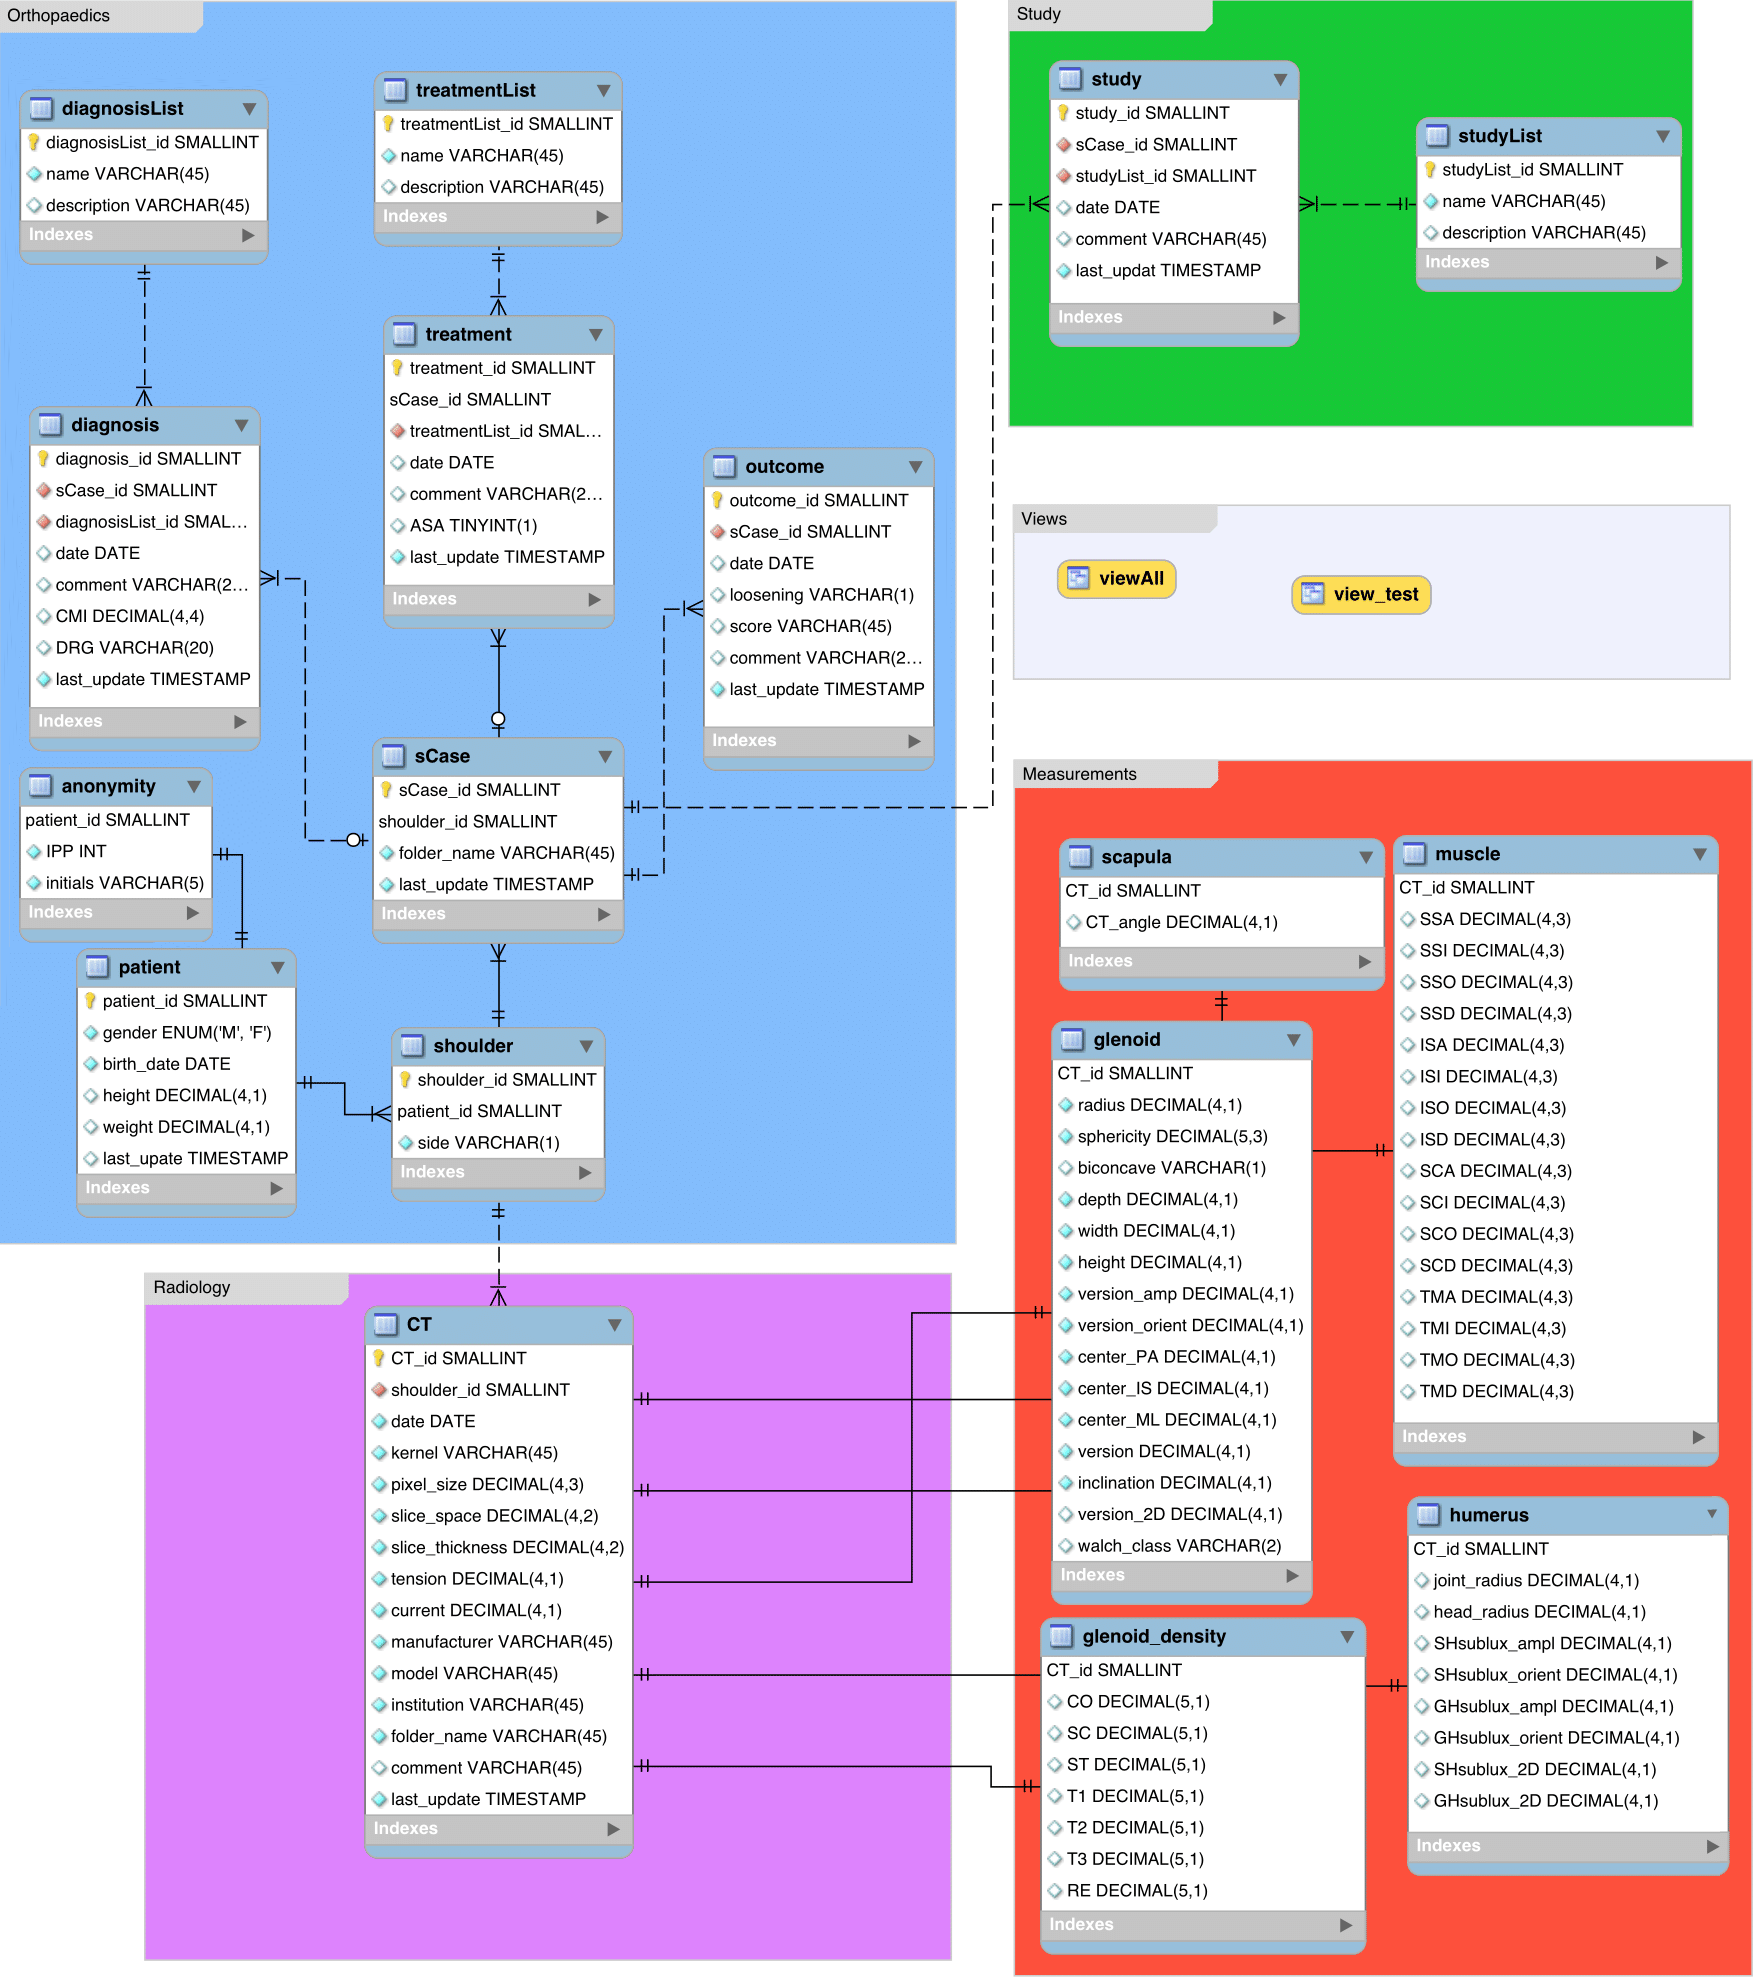
\includegraphics[width=1\textwidth]{images/analyse/SQLshoulderDatabase_reduced}
			\caption{Le schéma de la base de données reçu.}
			\label{schema_db}
		\end{figure}

		Nous allons donc prendre ce schéma comme référence pour la suite de l'analyse et du développement du projet.

	\subsection{Technologies}

		En plus de l'approche orientée utilisateur du projet, le but est également de découvrir et d'apprendre à utiliser certaines des plus récentes librairies du web. Pour ce projet, le choix logique a été fait de se concentrer une technologie servant à créer des interfaces utilisateur : React.

		Pour l'apprentissage de cette technologies et des librairies qui lui sont proches, j'ai suivi un tutoriel en plusieurs vidéo. Cette liste de vidéo est disponible sur YouTube\cite{learncode-academy}. 

		\subsubsection{React}\label{techno-react}
		
			\paragraph{Approche}

			Développée par Facebook le milieu de l'année 2013, React est "Une librairie JavaScript pour la création d'interfaces utilisateur"\cite{react}, traduit littéralement depuis le site officiel. React s'occupe donc strictement de la vue de l'application. Ce qui démarque principalement React des autres librairies similaires comme AngularJS est sa performance.

			La principale raison des performances élevées de React est dans le fait de conserver, en plus de la page affichée actuellement à l'écran (le DOM), un "DOM virtuel". Ce DOM virtuel est en pratique une copie en mémoire des éléments affichés à l'écran. La gestion habile de ce DOM virtuel permet à React de n'actualiser que les strictes parties de la page qui ont besoin de l'être, au moment où React le décide. Cela lui permet d'éviter beaucoup de rafraîchissements inutiles, que les autres librairies se devraient d'effectuer.

			\begin{figure}[h]
				\centering
				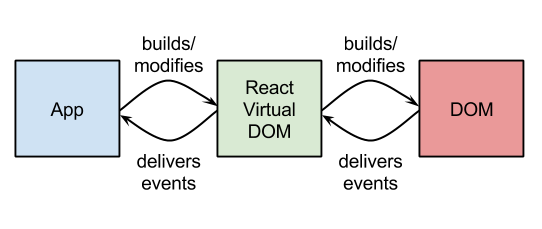
\includegraphics[width=0.8\textwidth]{images/analyse/virtualDOM}
				\caption{Le Virtual DOM est une étape intermédiaire entre React et le DOM\cite{valuecoders-choosereact}}
				\label{schema_virtualDOM}
			\end{figure}

			Le fait que le changement du DOM soit le principal élément lent dans presque tout code JavaScript permet donc à React de se démarquer.

			Une autres des caractéristiques de React est l'encouragement à écrire des composants réutilisables. De plus, bien que React ait été designé pour créer des interfaces web, il est aujourd'hui possible d'utiliser React ainsi que ses composants pour créer bien d'autres interfaces que du HTML. Par exemple, Facebook développe également depuis 2015 "React Native", qui permet d'utiliser des composants React pour créer des applications smartphone natives. Depuis, encore d'autres librairies ont constaté la puissance de React et tentent d'en tirer parti en dehors du navigateur.

			\paragraph{Tutoriel}

			Bien que React soit une librairie JavaScript, il est très recommandé de se construire un environnement de développement avec des outils adaptés afin de pouvoir développer correctement. Avec l'arrivée des gestionnaires de paquets tels que npm pour JavaScript, il serait une perte de temps de s'encombrer manuellement de toutes les étapes de recherche de dépendances de librairies, de leur assemblage, etc. Nous n'allons pas nous étendre sur tous les fichiers de configurations, mais allons lister les outils utiles pour React et allons expliquer la logique de fonctionnement principale de la librairie.

			\subparagraph{Node.js et npm}

			Nous allons partir du principe que la version 6.10.1 LTS de Node.js\cite{nodejs} (ainsi que npm\cite{npm}, qui est installé avec) sont installés sur la machine.

			Afin d'utiliser npm, nous allons créer un fichier de package, nommé 'package.json'. Ce fichier représente notre package d'application, et liste les librairies nécessaires pour le projet.

			\subparagraph{Dépendances}

			React lui-même est très puissant, mais il ne s'agit que du coeur logique du framework. D'autres librairies sont utilisées en cohésion avec React afin de par exemple générer du html. La figure~\ref{analyse_tutoriel_package}`montre' le contenu d'un fichier 'package.json' d'exemple, exposant des librairies quasi indispensables pour l'utilisation de React.

			\begin{figure}[!h]
				\begin{lstlisting}[]
{
  "name": "tutoriel",
  "version": "0.0.1",
  "description": "",
  "main": "webpack.config.js",
  "dependencies": {
    "react": "^15.4.2",
    "react-dom": "^15.4.2",
    "react-router": "^4.0.0",
    "react-router-dom": "^4.0.0-beta.8",
    "react-tap-event-plugin": "^2.0.1",
    "webpack": "^2.2.1",
    "webpack-dev-server": "^2.4.2"
  },
  "devDependencies": {},
  "scripts": {
    "dev": "webpack-dev-server --content-base src --inline --hot",
  },
  "author": "",
  "license": "ISC"
} \end{lstlisting}
				\caption{Fichier \texttt{package.json}}
				\label{analyse_tutoriel_package}
			\end{figure}

			On peut y voir les dépendances suivantes :

			\begin{itemize}
				\item \texttt{react} : Coeur logique de React.
				\item \texttt{react-dom} : Permet à React d'interagir avec le DOM.
				\item \texttt{react-router} : Permet à React d'interpréter des liens.
				\item \texttt{react-router-dom} : Fait le lien entre \texttt{react-router} et \texttt{react-dom}.
				\item \texttt{react-tap-event-plugin} : Corrige un bug pour que les interactions fonctionnent sur smartphone.
				\item \texttt{webpack} : Permet de "compiler" plusieurs scripts et librairies en un seul fichier JavaScript.
				\item \texttt{webpack-dev-server} : Permet de simplifier l'utilisation de \texttt{webpack} lors du développement.
			\end{itemize}

			\subparagraph{webpack et JSX}

			\texttt{webpack}\cite{webpack} est ici utile pour n'obtenir qu'un seul fichier JavaScript, très simple à utiliser avec une page HTML. Il est très recommandé de l'utiliser en cohésion avec React, mais son utilisation est optionnelle et sa configuration ne sera pas discutée ici. Les morceaux de code qui apparaîtront utiliseront tout de même la syntaxe JSX\cite{jsx}, qui est un sucre syntactique pour JavaScript. Il permet principalement d'écrire du code HTML dans du JavaScript. webpack, ainsi que d'autres technologies similaires, permettent de compiler cette syntaxe en JavaScript classique. Il est aussi tout à fait possible de ne pas utiliser JSX et d'écrire du JavaScript conventionnel simplement. La figure \ref{analyse_code_jsx} montre un code JSX, et la figure \ref{analyse_code_js} montre son équivalent JavaScript.

			\begin{figure}[!h]
				\begin{lstlisting}[language=html]
<MyButton color="blue" shadowSize={2}>
  Click Me
</MyButton> \end{lstlisting}
				\caption{Code JSX}
				\label{analyse_code_jsx}
			\end{figure}

			\begin{figure}[!h]
				\begin{lstlisting}[language=JavaScript]
React.createElement(
  MyButton,
  {color: 'blue', shadowSize: 2},
  'Click Me'
) \end{lstlisting}
				\caption{Equivalent compilé en JavaScript}
				\label{analyse_code_js}
			\end{figure}

			\subparagraph{Versions des librairies}

			Il est également à noter que React et d'autres librairies qu'il utilisent sont encore à ce jour énormément en développement, et il n'est pas rare de voir l'API changer, parfois excessivement souvent (j'ai pu voir des séries de changements conséquents à moins de 6 mois d'écart pour certaines librairies).

			Il est donc important de remarquer les versions utilisées des librairies, sur lesquelles se baseront à la fois le code du projet ainsi que ce guide d'utilisation. À noter également que les versions notées ici peuvent être utilisées ensemble, mais que cela n'est pas toujours le cas : Très souvent, une version d'une librairie va demander une version minimum d'une autre.

			\subparagraph{Composants}

			Le développement d'une application utilisant React repose sur la déclaration et l'utilisation de Composants. Un composant peut être vu comme un élément HTML possédant sa propre intelligence, indépendant des autres parties de la page. La figure \ref{analyse_composant_react} montre un exemple de code d'un composant simple.

			\begin{figure}[!h]
				\begin{lstlisting}[language=JavaScript]
class ShoppingList extends React.Component {
  render() {
    return (
      <div className="shopping-list">
        <h1>Shopping List for {this.props.name}</h1>
        <ul>
          <li>Instagram</li>
          <li>WhatsApp</li>
          <li>Oculus</li>
        </ul>
      </div>
    );
  }
}

// Example usage: <ShoppingList name="Mark" /> \end{lstlisting}
				\caption{Code d'un composant "\texttt{ShoppingList}", tiré de \cite{tutorial-react}}
				\label{analyse_composant_react}
			\end{figure}

			Voici les éléments qui constituent ici ce Composant :

			\begin{itemize}
				\item La méthode \texttt{render()} doit retourner une description de l'élément à afficher, soit ici un élément HTML (décrit avec la syntaxe JSX) en contenant plusieurs autres. Il s'agit là de la représentation qu'aura ce Composant lorsqu'il sera affiché dans la page HTML.
				\item Le paramètre \texttt{{this.props.name}}. Il s'agit là de code JavaScript : \texttt{this} se réfère à cette classe React, et \texttt{props} est un objet. \texttt{props} signifie 'propriétés', et c'est cet objet qui va généralement contenir les propriétés d'un élément React. Ici, une propriété est le nom \texttt{name}.
			\end{itemize}

			\subparagraph{Composition de Composants}

			Ici, le composant se constitue uniquement d'éléments HTML. Mais l'intérêt vient de la possibilité d'utiliser d'autres Composants à l'intérieur de la définition d'un de ces Composants. Par exemple, si nous avons décrit un Composant \texttt{Liste} dans notre code, nous pourrions l'utiliser ici à la place de l'élément HTML \texttt{ul} par exemple. Ainsi, la figure \ref{analyse_composant_react_2} montre cette modification apportée à notre décrit précédemment. 

			\begin{figure}[!h]
				\begin{lstlisting}[language=JavaScript]
class ShoppingList extends React.Component {
  render() {
    return (
      <div className="shopping-list">
        <h1>Shopping List for {this.props.name}</h1>
        <List values={['Instagram', 'WhatsApp', 'Oculus']}>
      </div>
    );
  }
}

// Example usage: <ShoppingList name="Mark" /> \end{lstlisting}
				\caption{Code modifié en utilisant un Composant}
				\label{analyse_composant_react_2}
			\end{figure}

			\subparagraph{Propriétés}

			Nous avons ici remplacé l'élément HTML par un composant fictif \texttt{<List>}. Celui-ci prend en paramètre une liste de valeurs. Dans notre cas, celles-ci seront ensuite passées à l'intérieur de son objet \texttt{props}, qu'il pourra faire usage pour afficher notre liste correctement.

			Nous sommes donc ici en possession d'un Composant fonctionnel très simple. Il serait tout à fait possible d'ajouter d'autres fonctionnalités à notre Composant : Il se comporte comme une Classe, et nous avons donc tout loisir de lui implémenter d'autres fonctions que l'actuel \texttt{render()} afin de le rendre réellement intelligent. De plus, React propose d'autres mécanismes que \texttt{props} pour faire interagir les composants entre eux, mais nous en savons déjà suffisamment pour comprendre le fonctionnement de base de React ici.

			\begin{figure}[!h]
				\begin{lstlisting}[language=HTML]
<html>
  <body>
    <div id="app"></div>
    <script src="script.js"></script>
    <script>
      ReactDOM.render(
        <ShoppingList />,
        document.getElementById('app')
      );
    </script>
  </body>
</html> \end{lstlisting}
				\caption{Code d'un fichier HTML affichant un Composant React.}
				\label{analyse_composant_react_3}
			\end{figure}

			\subparagraph{Affichage sur une page HTML}

			À présent, nous désirons afficher cet élément sur notre page HTML finale. En admettant que tout notre code (y compris les librairies \texttt{react} et \texttt{react-dom}) se trouve dans un fichier nommé \texttt{script.js} au même niveau qu'un fichier HTML, la figure \ref{analyse_composant_react_3} montre le code de la page nécessaire. Il suffit d'appeler la fonction \texttt{render} de \texttt{ReactDOM} en précisant en paramètres quel est l'élément principal à afficher, et où l'afficher sur la page.

			Maintenant que nous connaissons la logique principale de React et des Composants, nous pourrons nous intéresser à comment les composer intelligemment, et à utiliser des Composants autres que les nôtres.

		\subsubsection{Material-UI}

		Material-UI\cite{material-ui} est un ensemble de Composants React qui utilisent et respectent les guidelines de Google concernant Material Design\cite{material-design-guidelines}. L'utiliser va nous permettre de respecter facilement les guidelines de Material Design. Le but est de rendre le design la page cohérent dans son ensemble.

		\subsubsection{Flux}

		Flux\cite{flux} est un outil très souvent utilisé avec React, car son modèle le complète bien.
		Flux n'est pas vraiment un framework, mais plutôt un \gls{design pattern}.
		Flux définit une architecture d'application à suivre dans le code entier pour en tirer ses bénéfices, et propose quelques Classes pour implémenter son architecture proposée de manière rapide et facile.

		Contrairement au modèle MVC très souvent utilisé, Flux repose sur l'utilisation d'un flux de données unidirectionnel.

		\begin{figure}[h]
			\centering
			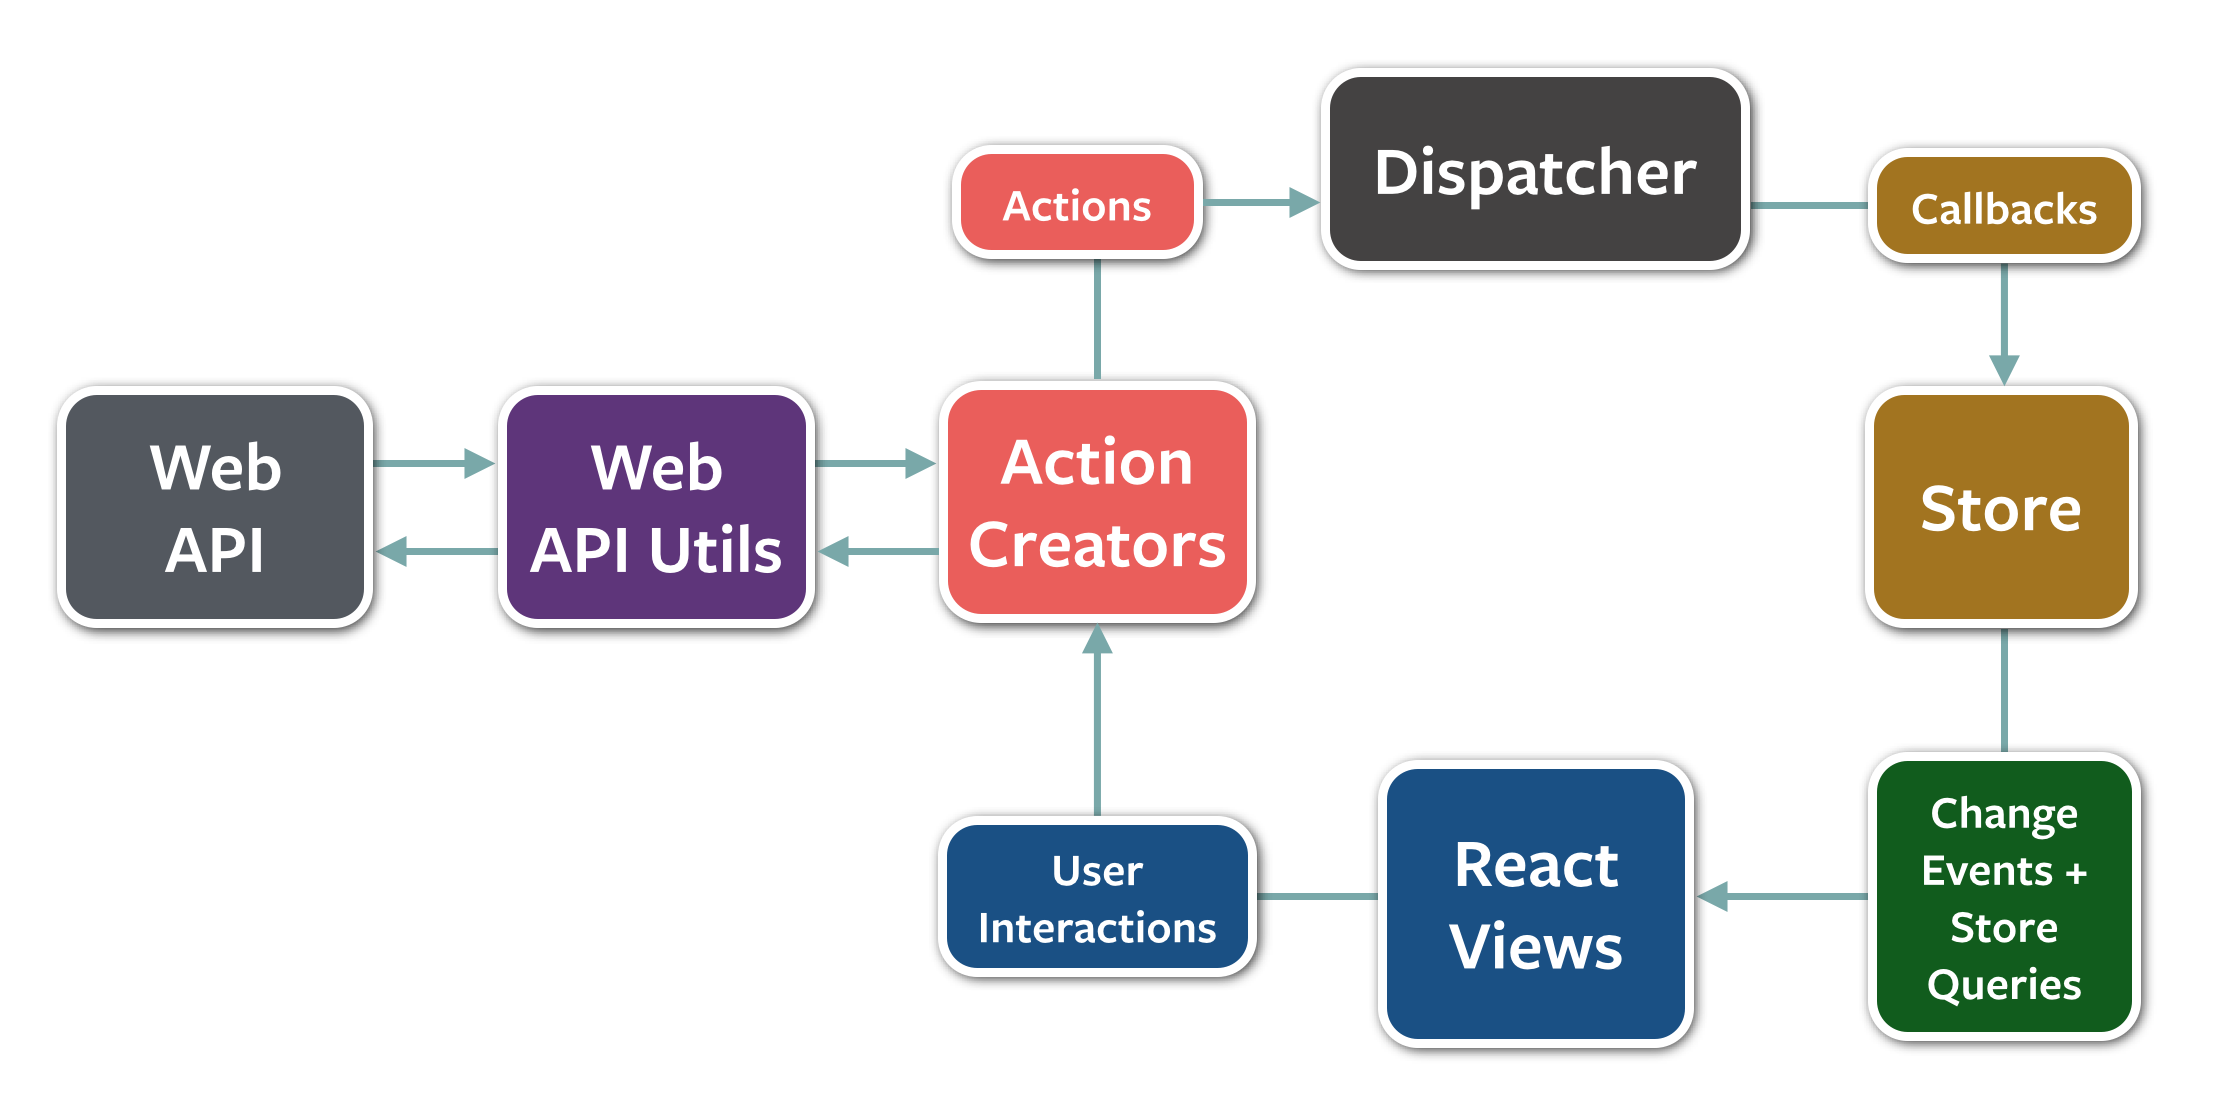
\includegraphics[width=1\textwidth]{images/analyse/flux}
			\caption{L'architecture que propose Flux est unidirectionnelle.\cite{flux-github}}
			\label{flux-diagram}
		\end{figure}

		La figure \ref{flux-diagram} montre un schéma de l'architecture que propose Flux. En plus des Composants React décrits précédemment, Flux se décompose en trois éléments principaux :

		\begin{description}
			\item[Stores] Un Store est un conteneur d'informations. Chaque Store va typiquement contenir un type d'information de la page web, et celui-ci devra être maintenu à jour. Il peut contenir par exemple le texte d'une conversation actuellement affichée. Les données contenues dans les stores vont souvent servir à être affichées sur la page web elle-même.
			\item[Actions] Une Action est ce qui est généré principalement par les choix de l'utilisateur. Il s'agit par exemple d'un clic sur un bouton, ou de la saisie d'un texte dans un champ.
			\item[Dispatcher] Le Dispatcher s'occupe de rassembler les Actions produites par les différents éléments de la page, et de les traiter afin d'envoyer des mises à jour aux Stores de la page pour que ceux-ci restent à jour.
		\end{description}

		\subsubsection{Backend}

			Plusieurs technologies seront utilisées du côté backend afin que l'application ne manque d'aucun composant.

			\paragraph{NodeJS}

			Node.js\cite{nodejs} permet d'exécuter des applications écrites en JavaScript en dehors du navigateur, sur une machine locale. Il sera utilisé ici en tant que serveur web pour répondre aux requêtes HTTP, et pour communiquer avec la base de données.

			\paragraph{Express}

			Express\cite{express} est une librairie JavaScript permettant d'écrire rapidement et facilement un serveur web.

			\paragraph{MySQL}

			MySQL\cite{mysql} est un système de gestion de bases de données. Son but est de conserver efficacement et de servir un grand nombre de données.
